% Indicate the main file. Must go at the beginning of the file.
% !TEX root = ../main.tex

%----------------------------------------------------------------------------------------
% CHAPTER TEMPLATE
%----------------------------------------------------------------------------------------


\chapter{Methodik} % Main chapter title

\label{Chapter3} % Change X to a consecutive number; for referencing this chapter elsewhere, use \ref{ChapterX}

%----------------------------------------------------------------------------------------
% SECTION 1
%----------------------------------------------------------------------------------------
In diesem Kapitel werden die Methoden und Vorgehensweisen zur Beantwortung der Forschungsfragen beschrieben. Das Ziel besteht darin, aussagekräftige Metriken zu extrahieren und Zusammenhänge festzustellen.
Zunächst wird die Erarbeitung der Forschungsfragen aufgezeigt, anschliessend die Vorgehensweise bei den Forschungsfragen. Dabei werden die Metriken vorgestellt, die untersucht werden sollen. Zusätzlich wird die für diese Arbeit wichtige Architektur aufgezeigt. Ebenso werden die Open-Source-GitHub-Projekte vorgestellt, die in Forschungsfrage 6 untersucht werden. Abschliessend wird die Datengrundlage präsentiert, auf der die Analysen basieren.

\section{Erarbeitung der Forschungsfragen}
\label{sec:ErarbeitungFF}
Die Forschungsfragen wurden im Rahmen der in \autoref{Chapter2} beschriebenen Literaturrecherche entwickelt. Dabei wurden Fachliteratur und Studien berücksichtigt, um relevante Metriken im Kontext von Pull-Requests und Code-Reviews zu identifizieren und miteinander zu vergleichen. Die Forschungsfragen wurden iterativ formuliert und kontinuierlich überarbeitet.

In der Literatur finden sich zahlreiche Metriken, die im Zusammenhang mit Pull-Requests untersucht werden. Besonders häufig analysiert werden dabei die Dauer (\textit{Latency}) und die Akzeptanz von Pull-Requests. Eine Übersicht dieser Metriken bietet \autoref{Chapter2}. Auffällig ist, dass einige Studien zu widersprüchlichen Ergebnissen hinsichtlich eines möglichen Zusammenhangs zwischen \textit{Latency} und \textit{Churn} (Anzahl geänderter Codezeilen) gelangen. Dieser Befund führte zur Formulierung der \fref{forschungsfrage1}, welche genau diesen Zusammenhang untersucht.

In vielen Studien werden hauptsächlich Open-Source-Projekte untersucht. Diese unterscheiden sich jedoch, wie in Kapitel \secref{sec:Projektmodule} und \secref{sec:OpenSourceProjekte} erläutert, in einigen Aspekten von den Projekten der Projektmodule, etwa hinsichtlich der Teamstruktur, Zielsetzung, Zeitplanung und des Erfahrungsniveaus der Contributor.
Aus diesem Grund wurden zunächst die spezifischen Rahmenbedingungen von Projekten der Projektmodule analysiert und anschliessend relevante Metriken definiert. Basierend darauf wurde die \fref{forschungsfrage6} formuliert, um die Unterschiede zwischen studentischen Projektmodulen und professionellen Open-Source-Projekten analysieren zu können.

Aus dieser Analyse ergeben sich die Forschungsfragen 3 bis 5, die sich mit dem Einfluss des Projektverlaufs, dem Arbeitsverhalten der Studierenden sowie den Unterschieden zwischen Teilzeit- und Vollzeitstudierenden befassen. Zusätzlich wurde die \fref{forschungsfrage2} formuliert, welche untersucht, ob sich die Schliessungsgründe von Pull-Requests in den Projekten identifizieren und klassifizieren lassen. Zudem soll geprüft werden, ob sich die in der Literatur erwähnten Metriken zur Akzeptanz auch auf diesen Kontext übertragen lassen. 

\section{Vorgehensweise bei den For\-schungs\-fragen}
\label{sec:AnalyseChurnvsLatency}
\label{sec:Metriken}
Um die Forschungsfragen beantworten zu können, musste das Mining von GitGauge erweitert werden. Dafür wurden weitere GraphQL-Abfragen implementiert und ein neuer Miner für Repositories erstellt sowie den Miner für Pull-Requests erweitert. Bei den Minern handelt es sich um sogenannte Extractor-Services, welche die GraphQL-Abfragen implementieren und die Daten in den entsprechenden Entitäten abspeichern.

Um die erste \fref{forschungsfrage1} beantworten zu können, müssen die Metriken \textit{Latency} und \textit{Churn} eingeführt werden. Die \textit{Latency} bestimmt die Zeitspanne zwischen der Eröffnung und der Schliessung eines Pull-Requests, sei es durch das Mergen des PRs oder durch manuelle Schliessung. Die manuelle Schliessung bedeutet, dass der Pull-Request entweder abgelehnt wurde oder durch den Autor des PRs erfolgte. Die \textit{Latency} wird anhand folgender Formel berechnet:
\begin{equation}
latency = closeTime - createTime
\end{equation}
Dabei handelt es sich bei den Metriken \textit{closeTime} und \textit{createTime} um zwei Metriken, die mittels Mining gewonnen werden können. Diese sind bereits im Pull-Request-Miner von GitGauge umgesetzt und mussten nicht neu implementiert werden. Bei den Namen der Metriken handelt es sich um die Namen der Attribute, wie sie in GitGauge genannt werden.

Des Weiteren wird die Metrik \textit{Churn} gebraucht. Diese Metrik setzt sich aus der Anzahl geänderter Zeilen im Pull-Request zusammen \parencite{gousios_exploratory_2014}. Folgend die Formel für \textit{Churn} (die Namen der Metriken werden von den Namen der Attribute in GitGauge abgeleitet): 
\begin{equation}
churn = additions + deletions
\end{equation}

Für die Metriken \textit{additions} und \textit{deletions} musste das Mining ebenfalls erweitert werden. Dazu wurde die bestehende Pull-Request-Entität um die Metriken \textit{additions} und \textit{deletions} ergänzt und im Miner für Pull-Request eine Abfrage via GraphQL erstellt. Die entsprechende GraphQL-Abfrage ist im folgenden \autoref{code:graphQLAdditionsDeletions} ersichtlich. Dabei konnten die Metriken direkt von der Pull-Request-Entität der entsprechenden GraphQL-Bibliothek (Octokit.GraphQL) bezogen werden.


\begin{lstlisting}[language=CSharp, caption={GraphQL-Abfrage additions und deletions}, label={code:graphQLAdditionsDeletions}]
var query = new Query()
.Repository(repositoryData.Repository!.Project, repositoryData.Repository!.Owner)
.PullRequests()
.AllPages()
    .Select(pr => new PullRequest
    {
        GitHubId = pr.Id.Value,
        Number = pr.Number,
        Title = pr.Title,
        Description = pr.BodyText,
        CreateTime = pr.CreatedAt,
        UpdateTime = pr.UpdatedAt,
        CloseTime = pr.ClosedAt,
    ......
}).Compile();
\end{lstlisting}

Um anschliessend den Zusammenhang der Metriken analysieren zu können, wird die Rangkorrelation nach Spearman verwendet \parencite{noauthor_t-test_nodate}. Mittels dieser kann überprüft werden, ob ein Zusammenhang zwischen zwei Variablen besteht. Dabei verwendet Spearman die Rangplätze der Daten und nicht deren Wert. Der daraus resultierende Korrelationskoeffizient r\textsubscript{s} kann zwischen -1 und 1 liegen, wobei dieser bei 1 einen starken positiven Zusammenhang und bei -1 einen starken negativen Zusammenhang zwischen den zwei Variablen darstellt. Wenn der Korrelationskoeffizient bei 0 liegt, besteht keine Korrelation. \parencite{noauthor_t-test_nodate}


Die Spearman-Formel \parencite{noauthor_t-test_nodate} stellt sich wie folgt zusammen: 
\begin{equation}
r_s = 1 - \frac{6 \sum d_i^2}{n(n^2 - 1)}
\end{equation}
\label{eqn:spearman}
\noindent\textbf{Legende:}
\begin{itemize}
  \item [$r_s$] Spearman-Rangkorrelationskoeffizient
  \item[$d_i$] Differenz der Ränge zwischen den zwei Variablen 
  \item[$n$] Anzahl der beobachteten Fälle
\end{itemize}

Zur Beantwortung der \fref{forschungsfrage2} ist der Status des Pull-Requests erforderlich. Ein Pull-Request kann entweder \textit{open} sein, wenn er noch aktiv ist, \textit{merged}, wenn er erfolgreich in den Zielbranch integriert wurde, oder \textit{closed}, wenn er ohne Merge geschlossen wurde \parencite{noauthor_enums_nodate}. Es sei darauf hingewiesen, dass diese Metrik nicht unmittelbar von GitHub extrahiert werden kann, sondern dass diese ermittelt werden muss. Dazu werden die Metriken \textit{closeTime} und \textit{mergeTime} benötigt. Im ersten Schritt wird überprüft, ob der PR  eine \textit{closeTime} aufweist. Ist dies der Fall, wird im zweiten Schritt überprüft, ob ebenfalls eine \textit{mergeTime} vorhanden ist. Somit kann evaluiert werden, ob der Pull-Request geschlossen wurde und ob dies durch ein Merging erfolgte. Diese Überprüfung ist bereits in GitGauge implementiert und wird entsprechend zur Beantwortung der \fref{forschungsfrage2} verwendet. Im Falle der \fref{forschungsfrage2} interessieren die Pull-Requests, die geschlossen, aber nicht gemergt wurden. Die Analyse der entsprechend geschlossenen PRs wurde manuell durchgeführt.

Bei \fref{forschungsfrage3} wird zusätzlich zu den bereits erwähnten Metriken \textit{createTime} und \textit{closeTime} des Pull-Requests die \textit{createTime} des Repositories benötigt, um berechnen zu können, zu welchem Zeitpunkt im Projekt ein Pull-Request erstellt oder geschlossen wurde.  Dafür wurde im neuen Repository-Miner die \textit{createTime } mittels GraphQL-Abfrage extrahiert. Dies ist im folgenden \autoref{code:graphQLRepoMiner} ersichtlich. Zudem wurde die Repository-Entität um das Erstellungsdatum erweitert. 
\begin{lstlisting}[language=CSharp, caption={GraphQL-Abfrage Repository}, label={code:graphQLRepoMiner}]
var repositoryQuery = new Query()
    .Repository(owner: repositoryData.Repository.Owner, name: repositoryData.Repository.Project)
    .Select(repo => new
    {
        repo.Name,
        repo.Owner.Login,
        repo.Description,
        repo.CreatedAt
    }).Compile();
\end{lstlisting}

Zusätzlich wurden die Abgabetermine der Projektmodule genutzt, um zu analysieren, wie weit ein Ereignis von der Abgabe entfernt erfolgte. Diese Termine wurden für die Projekte bereitgestellt und konnten nachgeschlagen werden.

Zur Identifizierung von Mustern in den Pull-Requests, die in der \fref{forschungsfrage4} thematisiert werden, erfolgt zusätzlich zu den Metriken \textit{createTime} und \textit{closeTime} eine Analyse der Commits auf den Pull-Requests. Zu diesem Zweck wurde die Pull-Request-Entität um die Commit-Entität erweitert. Die Commits beinhalten die Attribute \textit{Sha}, \textit{Message}, \textit{CommitTime} und \textit{Author}. Beim \textit{Sha} handelt es sich um den Hashwert des Commits, welcher als ID verwendet wird \parencite{noauthor_git_nodate}. Die \textit{Message} beinhaltet die Commit-Message, die bei einem Commit angegeben werden muss. Mittels der \textit{CommitTime} ist ersichtlich, wann der Commit gemacht wurde, und der \textit{Author} zeigt, wer den Commit gemacht hat. Zusätzlich musste die GraphQL-Abfrage im Pull-Request-Miner erweitert werden. Dies ist im \autoref{code:prCommits} ersichtlich. Dafür wurden aus der Pull-Request-Entität der GraphQL-Bibliothek die Commits ausgelesen und die entsprechenden Parameter abgefüllt.
\begin{lstlisting}[language=CSharp, caption={GraphQL-Abfrage Pull-Request-Commits}, label={code:prCommits}]
PullRequestCommits = pr.Commits(null, null, null, null)
    .AllPages()
    .Select(commit => new PullRequestCommitEntity()
    {
        PullRequestGraphqlId = commit.PullRequest.Id.Value,
        GitHubId = commit.Commit.Oid,
        Sha = commit.Commit.Oid,
        Message = commit.Commit.Message,
        CommitTime = commit.Commit.CommittedDate,
    }).ToList(),
\end{lstlisting}

\newpage
Die bereits aufgeführten Erweiterungen genügen für die Bearbeitung der \fref{forschungsfrage5}, sodass keine zusätzlichen Änderungen im Mining von GitGauge vorgenommen werden mussten. Jedoch mussten bei der Analyse die Klassen auf Vollzeit und Teilzeit aufgeteilt werden. In den Projektmodulen wird für jede Klasse jeweils eine GitHub-Organisation erstellt. Anhand der Namen dieser Organisationen kann erkannt werden, ob es sich um eine Teilzeit- oder Vollzeitklasse handelt, da der Klassenname darin vorkommt. Die Klassennamen für Informatik setzen sich wie folgt zusammen: 
\begin{equation}
IT<yy><Klassenkuerzel><Ort>
\end{equation}
\noindent\textbf{Legende:}
\begin{itemize}
  \item \textit{yy}: Die letzten zwei Ziffern des Jahres bei Studienbeginn (z.B. 23)
  \item\textit{Klassenkuerzel}: Bei Vollzeitklassen: a/b bei Teilzeit ta/tb
  \item\textit{Ort}: WIN/ZH (Abkürzungen für Winterthur und Zürich)
\end{itemize}

Anhand des Buchstabens \textit{t}'s kann somit erkannt werden, ob eine Klasse Teilzeit oder Vollzeit ist.

Für die \fref{forschungsfrage6} wurden sieben Metriken festgelegt, anhand derer die Korrelationsanalyse und der Vergleich mit OSS-Projekten stattfinden sollen. Die sieben Metriken sind: \textit{Latency}, \textit{Churn}, \textit{Commits}, \textit{Comments}, \textit{Description Length}, \textit{Changed Files Count} und \textit{Contributors}. Diese wurden, wie in Kapitel \secref{sec:ErarbeitungFF} erwähnt, durch Literaturrecherche festgelegt. Die entsprechenden Metriken werden im folgenden Abschnitt \secref{sec:MetrikenKorrelation} aufgezeigt und die entsprechenden OSS-Projekte werden im Kapitel \secref{sec:VorstellungGithubOrgs} vorgestellt. Für die Korrelationsanalyse musste das Mining erweitert werden. Zusätzlich zu den bereits genannten Erweiterungen wurden noch die Metriken \textit{ChangedFiles} und \textit{TotalCommits} extrahiert.

Die Analysen der Forschungsfragen erfolgten via Jupyter-Notebooks. Für die einzelnen Untersuchungen wurde jeweils ein neues Jupyter-Notebook erstellt. Diese ermöglichen eine schnelle und unkomplizierte (grafische) Auswertung der Daten. \parencite{noauthor_repo-detectivesba-metric-analysis-scripts_nodate}


\section{Metriken für die Korrelations\-analyse}
\label{sec:MetrikenKorrelation}
Für die Korrelationsanalyse der Metriken zur Klärung von \fref{forschungsfrage6} müssen geeignete Metriken ausgewählt werden, die verschiedene Aspekte der Pull-Request-Dynamik abbilden. Soziale Faktoren wie die Erfahrung der Contributor oder die Dauer ihrer Mitarbeit an einem Projekt können jedoch nicht berücksichtigt werden, da solche Daten im Kontext der untersuchten Studenten-Repositories nicht verfügbar sind. Basierend auf der Analyse diverser wissenschaftlicher Literatur wurden folgende sieben Metriken ausgewählt:

Als \textbf{Latency} wird die Zeit zwischen der Erstellung eines Pull-Requests und dessen Merge oder Schliessung genannt. Sie wird als Indikator für die Effizienz des Review-Prozesses genutzt und ist in der Literatur häufig als Schlüsselfaktor für die Messung der Geschwindigkeit von Code-Reviews und DevOps-Prozessen anerkannt. Eine hohe Latenz kann auf ineffiziente Reviews oder Verzögerungen hinweisen, weshalb sie in die Analyse aufgenommen wurde, um die Geschwindigkeit der Pull-Request-Bearbeitung zu messen und Zusammenhänge mit anderen Metriken wie \textit{Churn} und \textit{Comments} zu untersuchen. \parencite{yu_wait_2015}

Die Metrik \textbf{Churn} misst die Anzahl geänderter Codezeilen in einem Pull-Request. Sie wird als Indikator für den Umfang und die Komplexität einer Änderung betrachtet und ist häufig mit längeren Review-Zeiten verbunden. Diese Metrik wurde ausgewählt, da grössere Änderungen im Code oft genauere Überprüfungen erfordern und somit die \textit{Latency} des Pull-Requests beeinflussen können. \parencite{gousios_exploratory_2014}

Die Anzahl der \textbf{Commits} in einem Pull-Request gibt an, wie viele Commits gemergt werden sollen. Sie zeigt, wie kleinschrittig oder iterativ ein Beitrag entwickelt wurde. Mehrere Commits deuten häufig darauf hin, dass der Pull-Request mehrere Anpassungen durchlaufen hat, was zu einer längeren Review-Dauer führt. \parencite{zhang_pull_2022}

\textbf{Comments} messen die Anzahl der Kommentare, die während des Review-Prozesses als auch auf den Pull-Request selber erstellt wurden. Eine höhere Anzahl an Kommentaren deutet auf intensivere Diskussionen hin, die den Review-Prozess verlängern können und die Wahrscheinlichkeit eines Merges verringern. Zudem ist eine hohe Zahl an Kommentaren oft mit einer höheren Qualität und Gründlichkeit des Reviews verbunden. \parencite{tsay_influence_2014}

Die Länge der Beschreibung eines Pull-Requests (\textbf{Description Length}) ist ein Indikator für den Kontext, den der Entwickler für seine Änderungen liefert. Ausführliche Beschreibungen helfen den Reviewern, die Änderungen schneller zu verstehen, was den Review-Prozess beschleunigen kann. Kürzere Beschreibungen führen häufig zu mehr Rückfragen und somit zu einer längeren Review-Dauer. \parencite{zhang_pull_2022}

Neben der Anzahl geänderter Codezeilen gibt \textbf{Changed Files Count} an, wie viele Dateien von einer Änderung betroffen sind. Diese Metrik ist wichtig, da Änderungen, die viele Dateien betreffen, in der Regel komplexer sind und daher länger dauern, um überprüft und integriert zu werden. \parencite{tsay_influence_2014}

Die Metrik \textbf{Contributors} misst die Anzahl der verschiedenen Entwickler, die an einem Pull-Request beteiligt sind. Ein höherer Beitrag von verschiedenen Entwicklern könnte auf eine intensivere Zusammenarbeit hinweisen und könnte mit der Komplexität und der Dauer des Review-Prozesses korrelieren.

\section{Erkennung Git-Squashing}
\label{sec:ErkennungSquashing}
Mit \textit{Git-Squashing} können mehrere Commits zu einem Commit zusammengeführt werden, bevor diese in den Zielbranch gemergt werden. Die theoretischen Grundlagen werden in \secref{sec:GitSquashing} erläutert. 

Um das neue Feature in GitGauge zu implementieren, müssen gesquashte Commits erkannt und optional berücksichtigt werden. Ziel der neuen Implementierung ist es, sichtbar zu machen, wann genau Contributors Commits erstellen, um daraus ableiten zu können, an welchen Tagen aktiv gearbeitet wurde. Damit dieses Bild möglichst akkurat ist, sollen nicht nur die Commits im Haupt-Branch (Main / Master-Branch) berücksichtigt werden, sondern auch jene Commits, die ursprünglich in Pull Requests enthalten waren, aber durch Squashing beim Merge zu einem einzelnen Commit zusammengefasst wurden.

Das Herausfiltern von gesquashten Commits ist hierbei essenziell, da Squashing die Metriken über die tatsächliche Arbeitsverteilung verfälschen kann. Betrachtet man lediglich diesen finalen Merge-Commit, so gehen wesentliche Informationen verloren. Beispielsweise darüber an welchen Tagen tatsächlich entwickelt wurde, wie kontinuierlich die Arbeit stattfand und wie viele Einzelschritte zum Endergebnis führten. Der Squash-Commit bildet lediglich den Merge-Zeitpunkt ab und verschleiert so die zeitliche Struktur der Entwicklung. 

Um dem entgegenzuwirken, bietet die neue Implementierung eine Einstellungsmöglichkeit, mit der gesquashte Feature-Commits optional in die Auswertung einbezogen werden können. Über einen entsprechenden Toggle (\textit{Include Squashed Feature Commits}) kann diese Option aktiviert oder deaktiviert werden. Je nach Einstellung des Feature-Toggles wird die Datenverarbeitung wie folgt angepasst:
\begin{itemize}
    \item \textbf{Feature deaktiviert}: Es werden ausschliesslich die Commits aus dem Main-Branch berücksichtigt. Gesquashte Commits aus Feature-Branches werden als ein Commit analysiert.
    \item \textbf{Feature aktiviert}: Zwei Filter- und Einbeziehungsschritte werden vorgenommen:
        \begin{itemize}
        \item Gesquashte Commits auf dem Main-Branch werden ausgeschlossen.
        \item Alle Commits aus den gesquashten Feature-Branches werden in die Analyse integriert.
    \end{itemize}
\end{itemize}

Die nicht gesquashten Pull-Requests müssen dabei nicht inkludiert werden, da die gesamte Feature-Branch-Historie auf dem Main-Branch vorhanden ist. 

\autoref{lst:graphql-commits} zeigt die Logik zur Verarbeitung gesquashter Commits in der Methode \textit{GetCommitsCountPerDate} der Klasse \textit{ContributorMetricsCalculator}. Diese Vorgehensweise wurde konsistent in allen Methoden hinzugefügt, welche zur Berechnung der Graphen erforderlich sind.

\begin{lstlisting}[language=CSharp, caption={Verarbeitung gesquashter Commits in der Methode \textit{GetCommitsCountPerDate}}, label={lst:graphql-commits}]
void processCommit(DateTime commitDate, ContributorDto contributor)
{

	if (!commitsCountPerDate.ContainsKey(commitDate))
	{
		commitsCountPerDate[commitDate] = new Dictionary<String, int>();
	}

	if (!commitsCountPerDate[commitDate].ContainsKey(contributor.Username))
	{
		commitsCountPerDate[commitDate][contributor.Username] = 0;
	}

	commitsCountPerDate[commitDate][contributor.Username]++;
}
foreach (Commit commit in commits)
{
	// skip squashed commits if feature commits should be included instead
	if (queryParams.IncludeSquashedFeatureCommits && squashedCommits.Contains(commit.Sha))
	{
		continue;
	}
	processCommit(commit.CommitTime.Date, commit.Author!.ToContributorDto());
}


if (queryParams.IncludeSquashedFeatureCommits)
{
	foreach (PullRequest pr in pullRequests)
	{
		if (IsPullRequestToMainSquashed(pr, commits))
		{
			foreach (PullRequestCommitEntity commit in pr.PullRequestCommits)
			{
				processCommit(commit.CommitTime.Date, commit.Author!.ToContributorDto());;		
			}	
		}
	}
}

return commitsCountPerDate;
\end{lstlisting}

Der in \autoref{lst:graphql-commits} dargestellte Code implementiert die Zählung von Commits pro Contributor und Datum, wobei optional auch gesquashte Feature-Commits berücksichtigt werden können. Die gezeigte Methode nutzt dazu die Hilfsmethode \textit{processCommit}, welche die Zählwerte in einer verschachtelten Dictionary-Struktur (\textit{commitsCountPerDate}) aggregiert.

Zuerst werden alle Commits des Main-Branches verarbeitet. Ist die Option \textit{IncludeSquashedFeatureCommits} aktiviert, so werden gesquashte Commits aus dem Main-Branch übersprungen. In einem zweiten Schritt werden alle Pull-Request-Commits, welche den Main- / Master-Branch als Target besitzen, in die Liste miteinbezogen. 

\newpage
\section{Architektur}
Die \autoref{fig:Vereinfachte_Architektur} zeigt eine vereinfachte Architektur der GitGauge-Applikation. Sie beschränkt sich auf die wesentlichen Komponenten, die im Rahmen der Forschungsarbeiten benötigt werden. Dabei sind die in der Arbeit verwendeten und erweiterten Komponenten von GitGauge dargestellt. Ausserdem wird der in der Arbeit entwickelte Analyser aufgezeigt, der ausserhalb der GitGauge-Applikation existiert und lediglich die Daten von GitGauge bezieht.  
\begin{figure}[htbp]
    \centering
    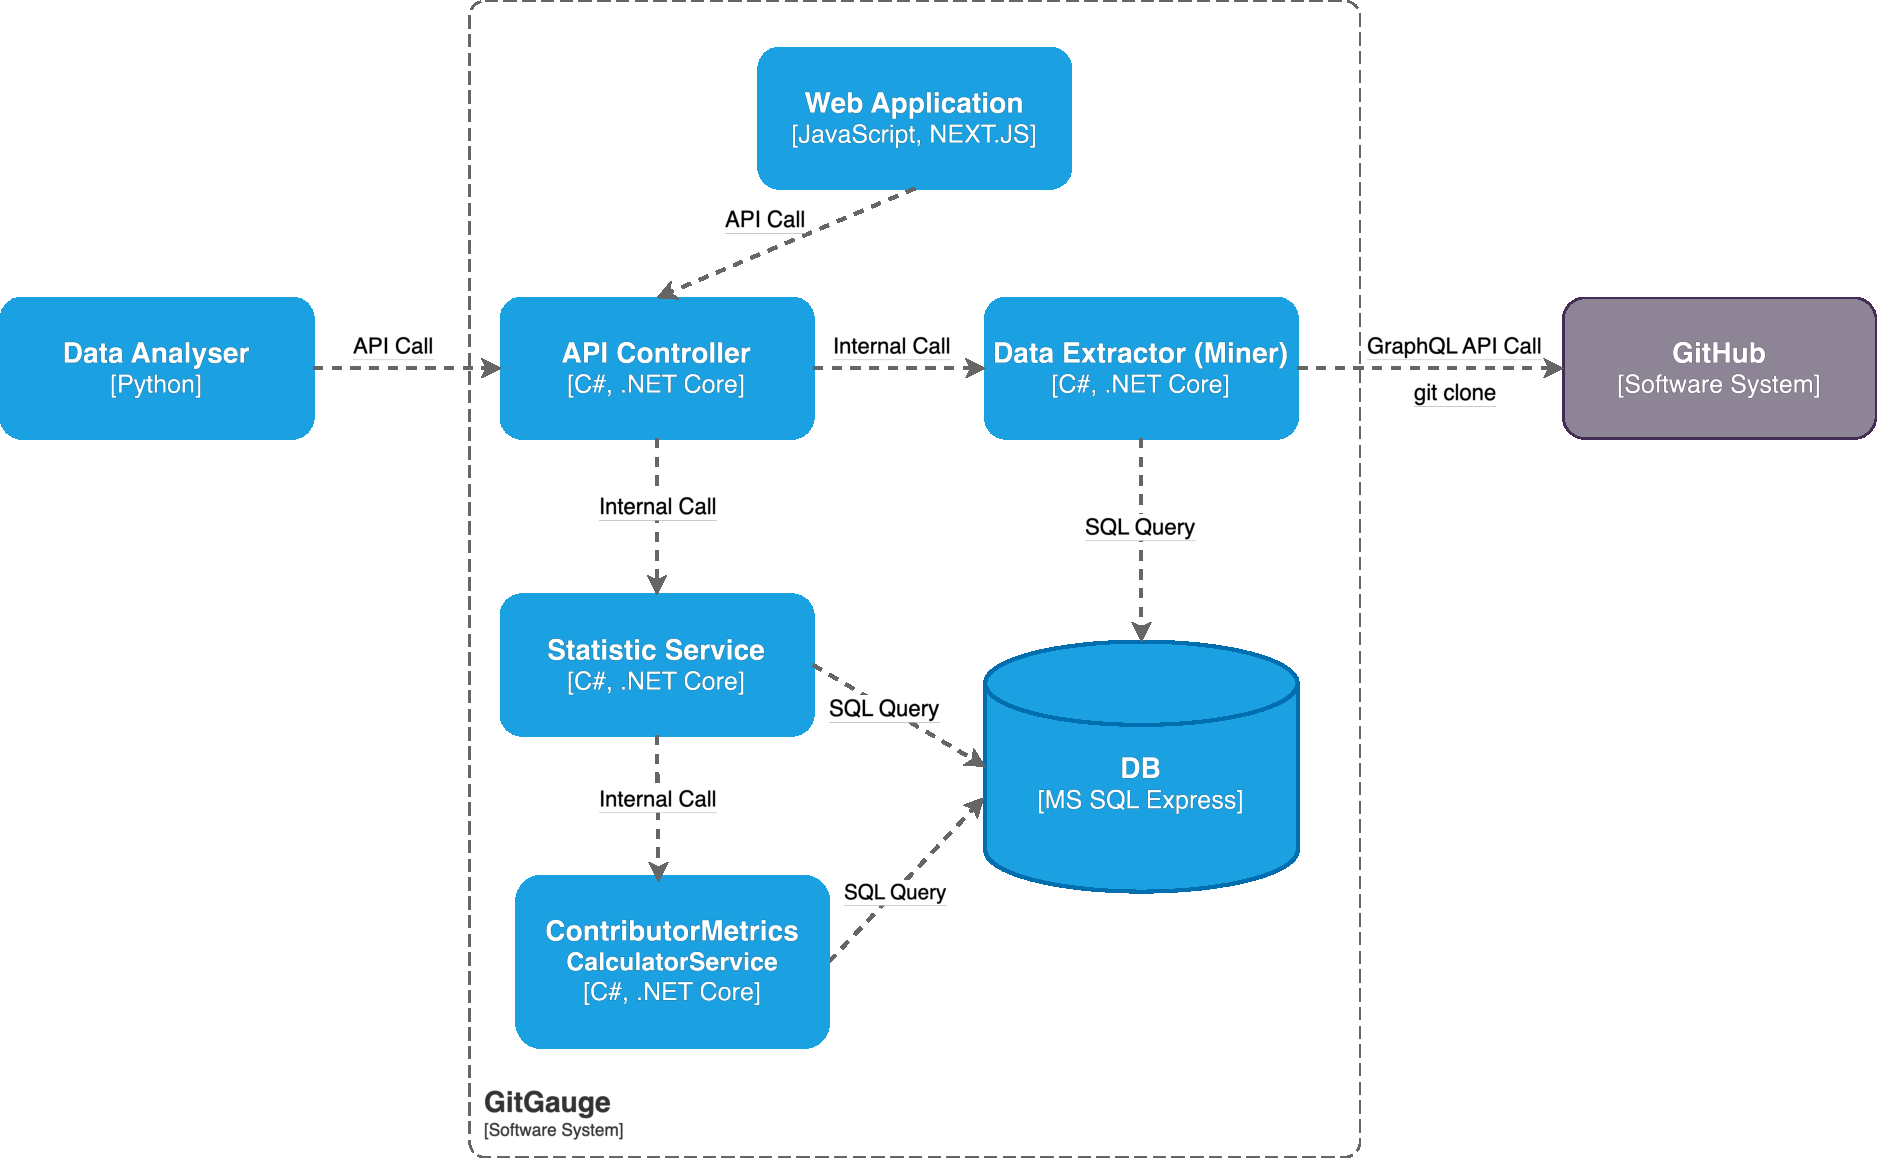
\includegraphics[width=0.8\textwidth]{Figures/Vereinfachte_Architektur.pdf}
    \caption{Architektur}
    \label{fig:Vereinfachte_Architektur}
\end{figure}

Im Folgenden werden die Komponenten beschrieben:
\begin{itemize}
    \item \textbf{GitHub}: GitHub dient als externe Datenquelle und stellt über die GraphQL-API sowie durch das Klonen von Repositories-Informationen zu Metriken wie Repositories, Commits und Pull-Requests bereit.
    \item \textbf{DB}: Die Datenbank (MSSQL Express) dient der Applikation als zentrales Speichermedium. In der relationalen Datenbank werden die extrahierten Metriken gespeichert. 
    \item \textbf{Data Extractor (Miner)}: Die Data Extractor-Services sind in C\# .NET Core geschrieben und implementieren das Interface \textit{IDataExtractorService}. In diesen Services wird der Mining-Prozess durchgeführt. Die Datenabfrage in den einzelnen Services erfolgt entweder über die GraphQL-API oder durch das Klonen von Git-Repositories. Das Ergebnis der Abfragen wird anschliessend jeweils von dem entsprechenden Service in die Datenbank geschrieben. 
    \item \textbf{API Controller}: Auch die API Controllers sind in C\# .NET Core implementiert. Sie aggregieren Daten aus der Datenbank und stellen diese über REST-Schnittstellen den konsumierenden Komponenten zur Verfügung. Darüber hinaus nehmen die Controller neue Mining-Anfragen entgegen und leiten diese an den Data Extractor weiter.
    \item \textbf{Statistic Service}: Der Statistic Service ist in C\# unter .NET Core implementiert und stellt mehrere Methoden zur Analyse von Repository-bezogenen Metriken bereit. Im Rahmen der Erweiterung für die Forschungsfragen wurde der Service um die Methode \textit{GetContributorsStatisticsAsync} erweitert, welche Beitragsstatistiken von Mitwirkenden eines Repositories ermittelt. Diese Statistiken geben Auskunft über die zeitliche Verteilung von Commits pro Tag sowie deren Häufung pro Wochentag. Grundlage hierfür sind Commit- und Pull-Request-Daten, die aus der Datenbank geladen und durch den \textit{ContributorMetricsCalculator} aufbereitet werden.
    \item \textbf{ContributorMetricsCalculator}: Der ContributorMetricsCalculator ist eine Hilfsklasse innerhalb des Statistic Service. Sie verarbeitet Commit-Daten, um verschiedene Metriken zur Beitragsaktivität von Entwicklern zu berechnen. Dieser Service wurde um mehrere Methoden erweitert, welche die Anzahl der täglichen Commits pro Entwickler sowie deren Verteilung über die Wochentage auswertet. Die Berechnung der Metriken kann mittels Parameter angepasst werden. 
    \item \textbf{Web Application}: Die Webanwendung wurde mit Next.js entwickelt. Sie dient GitGauge-Anwendern als Einstiegspunkt. Über sie können Analysen zu den Repositories dargestellt, neue Repositories erfasst und Aufträge fürs Mining erstellt werden. 
    \item \textbf{Data Analyser}:  Der in Python implementierte Data Analyser dient der weiterführenden Auswertung und Interpretation der gesammelten GitHub-Daten. Über den API-Controller ruft er relevante Informationen ab, verarbeitet sie mithilfe von Algorithmen der Datenanalyse und liefert aggregierte oder statistische Ergebnisse zurück. Diese werden zusätzlich visuell aufbereitet.
\end{itemize}

\section{Erweiterung GitGauge Web Application}
Aufgrund der Analysen, die für die \fref{forschungsfrage4} durchgeführt wurden, stellte sich die Metrik der Commits pro Contributor als eine interessante Grundlage für eine Erweiterung der GitGauge Web Application heraus.  
Ziel der Erweiterung ist es, die Arbeitszeiten der Teammitglieder anzuzeigen. Dies soll den Dozierenden dabei helfen, Probleme bei der Zusammenarbeit der Studierenden zu erkennen und zu analysieren, ob es beispielsweise ungleiche Arbeitsverteilungen oder Verzögerungen gibt.

\subsection{Erkennung Arbeitszeiten}
Die Arbeitszeiten der Teammitglieder werden anhand der Commits innerhalb der Projekte ermittelt. Dabei muss berücksichtigt werden, dass der Main-Branch nicht alle Commits beinhaltet. Feature-Branches können noch nicht gemerged sein oder die Metrik kann durch \textit{squashed Commits} verfälscht werden. Um dennoch alle Commits analysieren zu können, werden zusätzlich alle Pull-Requests eingelesen, welche den Main-/Master-Branch als Target besitzen und alle aufgelisteten Commits in die Analyse integriert. Dies wird im Abschnitt \secref{sec:ErkennungSquashing} erläutert.

\subsection{Implementierung}
Zusätzlich zum Mining der Pull-Request Commit-Daten werden die Daten aggregiert und dem Frontend zur Verfügung gestellt. Dazu wurde ein neuer Endpoint erstellt, der die Daten sowohl datumsbasiert als auch wochentagsbasiert pro Benutzer (Contributor) ausgibt. Diese Daten werden dann im Frontend aufbereitet und visualisiert. Dazu wird mithilfe der MUI X-Library zwei Grafiken erstellt \parencite{noauthor_react_nodate}. Diese zeigen, wie in \autoref{fig:gitgauge_commits} ersichtlich, zum einen die Commits pro User basierend auf Datum und zum anderen die Commits pro User pro Wochentag. Mittels des Switches in der linken oberen Ecke können entweder nur die Commits auf dem Main-Branch angezeigt werden oder zusätzlich zu den Commits auf dem Main auch noch die Pull-Request Commits, welche mit einem Squashed-Commit auf den Main-Branch gemerged wurden.

Das erste Diagramm ermöglicht den Benutzern des Tools einen allgemeinen Überblick über die Arbeitsaktivitäten der Teammitglieder. Es erlaubt Rückschlüsse darauf, ob alle Mitglieder während der gesamten Projektlaufzeit kontinuierlich zum Projekt beigetragen haben.

Die zweite Grafik zeigt, an welchen Wochentagen die Projektarbeit stattfindet. Dadurch lässt sich analysieren, ob die Arbeitsverteilung innerhalb des Teams ausgewogen ist oder ob signifikante Unterschiede bestehen, die potenziell zu Konflikten in der Zusammenarbeit führen können.

Die \autoref{fig:gitgauge_commits} zeigt die Auswertung eines Racetrack-Repositorys. Um die Privatsphäre der Studierenden zu gewährleisten, werden die Daten anonymisiert dargestellt. Anhand des ersten Diagramms ist zu erkennen, dass kontinuierlich an dem Projekt gearbeitet wurde und alle Teammitglieder ihren Beitrag geleistet haben. Das Projektende scheint am 24.03.2022 gewesen zu sein, die Aktivität am 14.04.2022 war das Feedback des Dozenten. Im zweiten Diagramm ist zu sehen, dass die Studierenden vor allem an den Tagen Mittwoch und Donnerstag gearbeitet haben. Ebenfalls ist zu sehen, an welchen Wochentagen die jeweiligen Studierenden bevorzugt gearbeitet haben.
\begin{figure}[htbp]
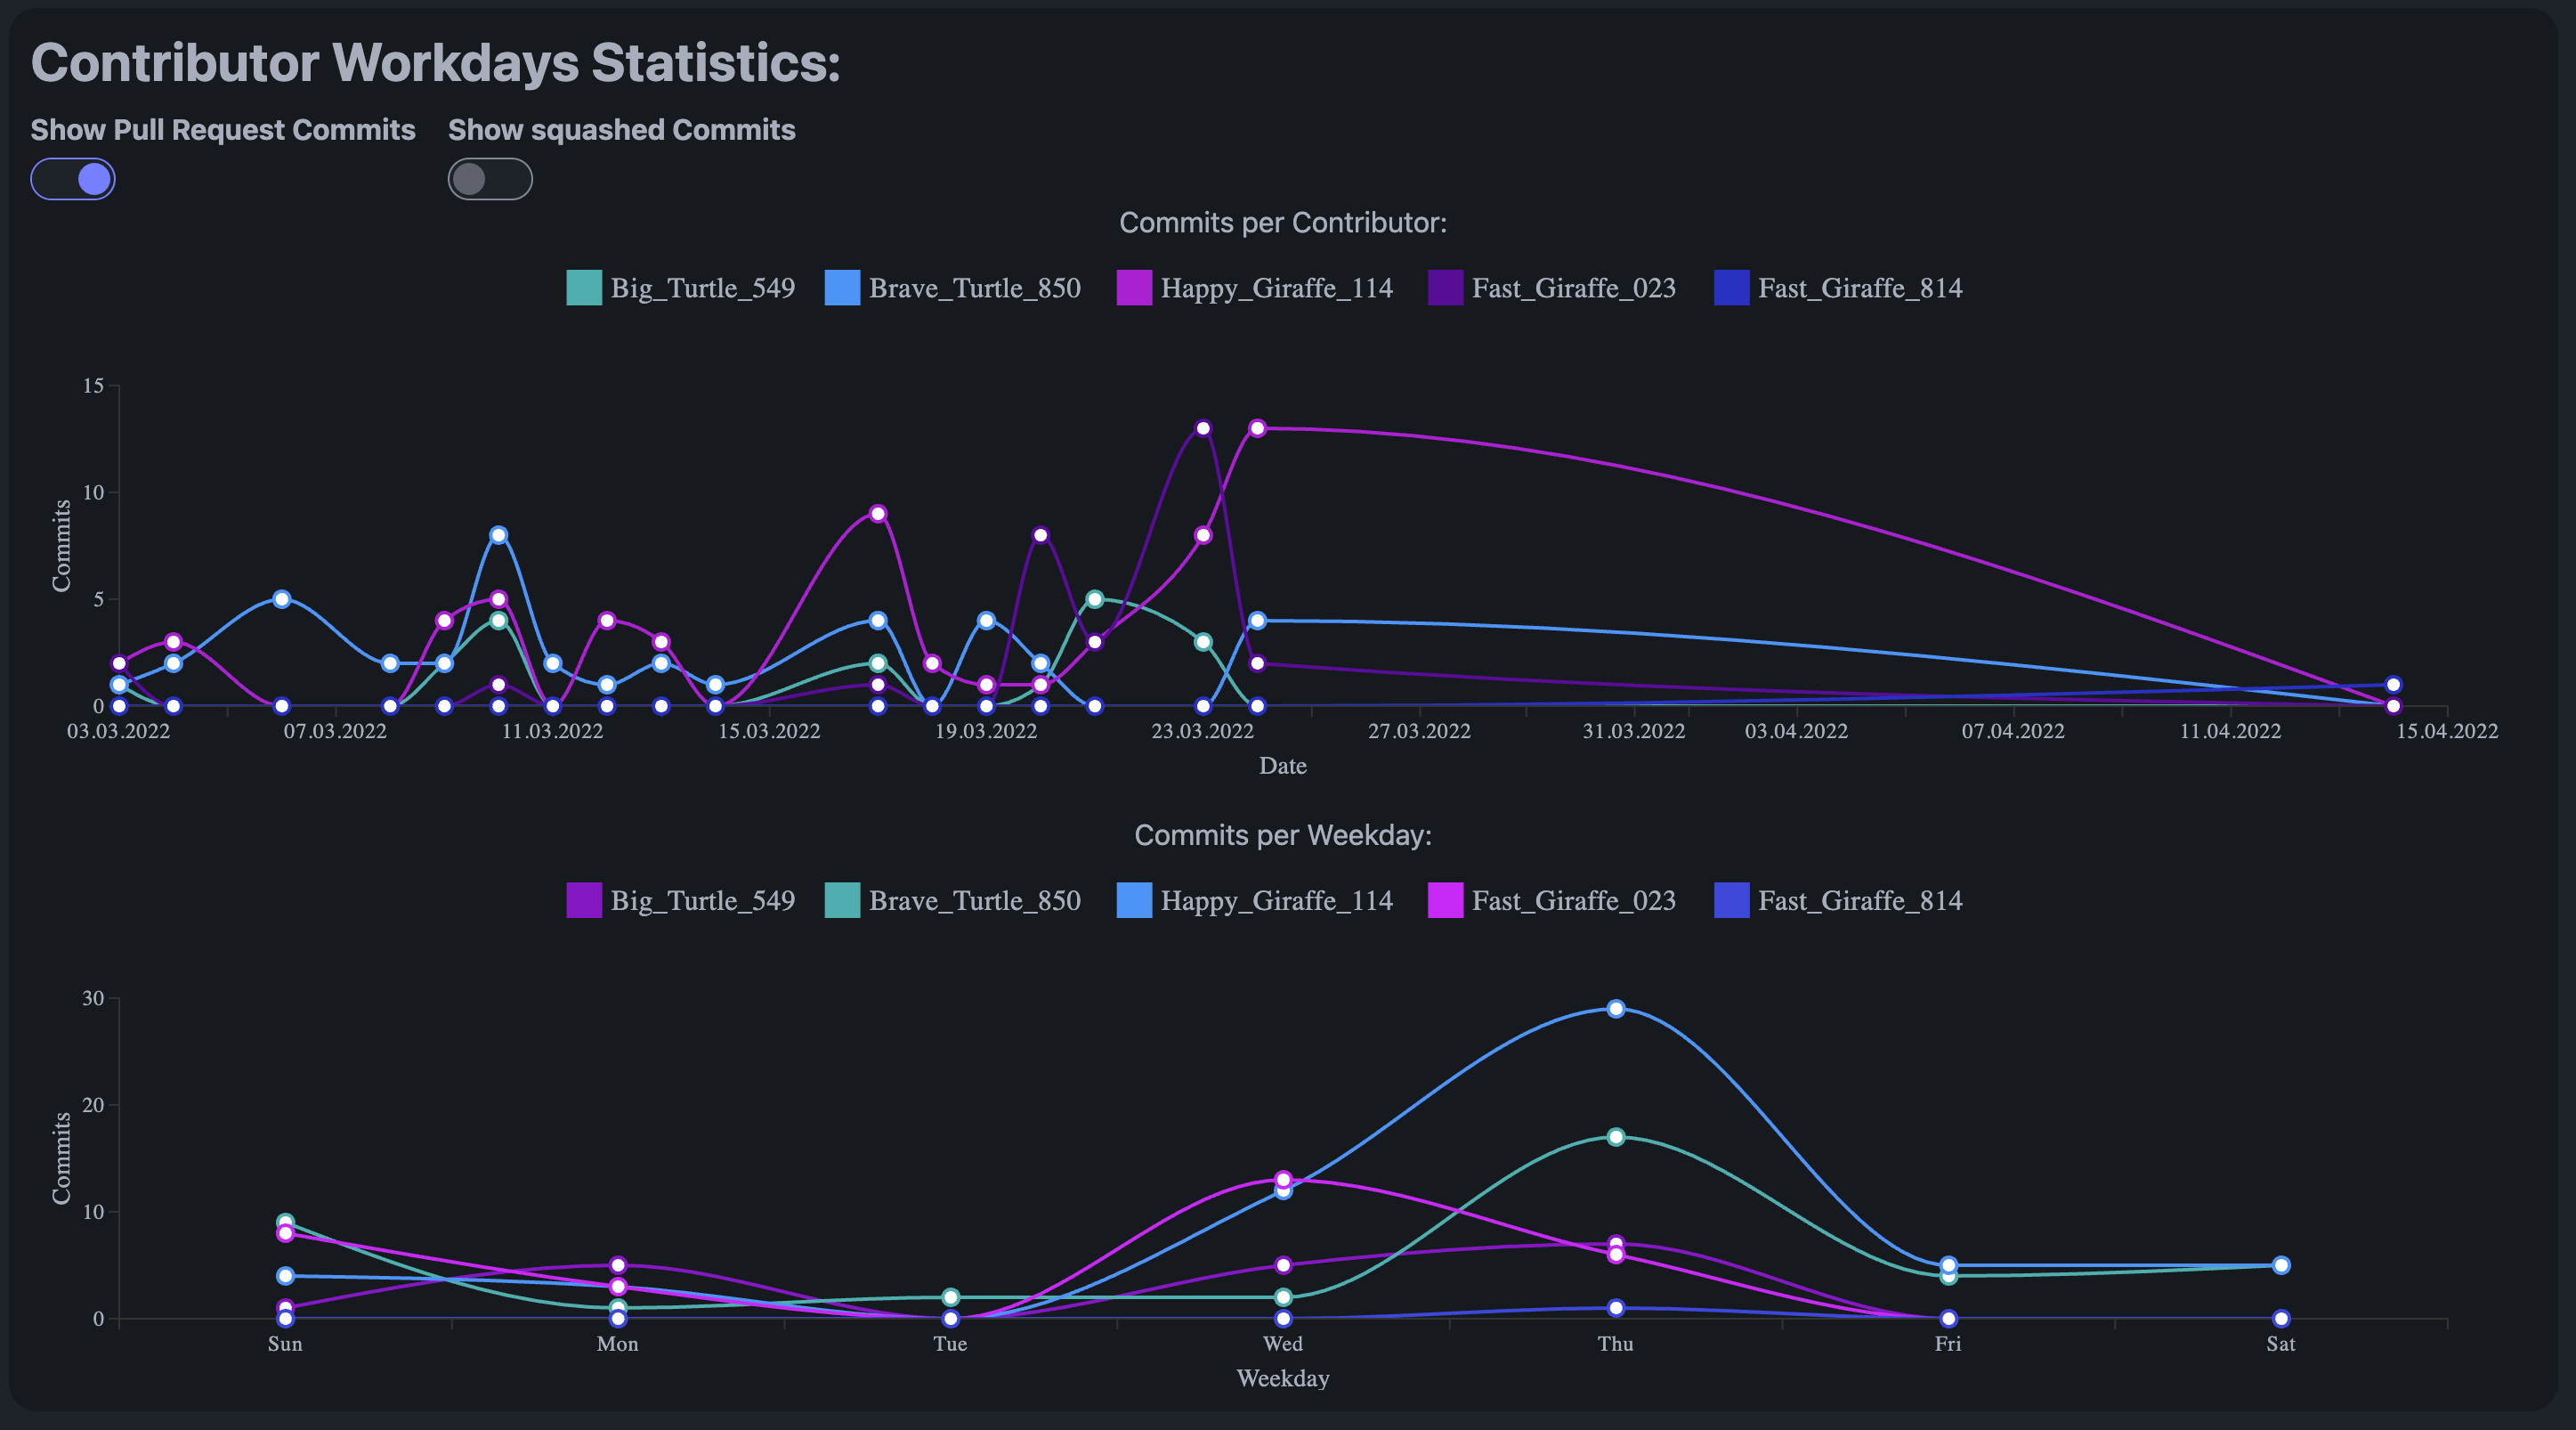
\includegraphics[width=\textwidth]{Figures/gitgauge_commits.png}
\caption{GitGauge Implementierung der \textit{Commit per User} Darstellung }
\label{fig:gitgauge_commits}
\end{figure}



\section{Datengrundlagen}
\label{sec:Datengrundlagen}
Als Datengrundlage dienen die Repositories aus dem Racetrack Projekt, welches im zweiten Projektmodul stattfindet. Dieses dauert etwa vier Wochen, wobei die genaue Anzahl der Tage pro Klasse variieren kann. Das Grundgerüst des Sourcecodes wird in der Aufgabenstellung mitgeliefert, was die Vergleichbarkeit der Projekte erhöht. Es werden 7 Teilzeit- und 5 Vollzeitklassen aus den Jahren 2021 - 2024 analysiert. Insgesamt werden 71 Racetrack-Repositories untersucht. 

\subsection{Vorstellung der GitHub-Organisationen}
\label{sec:VorstellungGithubOrgs}
Für den Vergleich der Korrelationsanalyse der Racetrack-Repositories werden drei GitHub-Organisationen ausgewählt. Diese unterscheiden sich in ihrer Unternehmensgrösse, der Anzahl ihrer Projekte, der Grösse der jeweiligen Projekte sowie im Anteil der Repositories, die nicht nur öffentlich zugänglich sind, sondern auch aktiv als Open-Source-Projekte mit Beiträgen externer Contributor weiterentwickelt werden.

\textit{Ubique Innovation AG} ist ein Schweizer Unternehmen mit Sitz in Zürich, das sich auf die Entwicklung von Softwarelösungen mit Fokus auf Mobile-App-Entwicklung spezialisiert hat. Im Jahr 2021 beschäftigte die Firma rund 50 Mitarbeiter \cite{noauthor_mathias_2021}. Zu den bekanntesten Projekten von Ubique gehören unter anderem die Mobile-App der Schweizerischen Bundesbahnen (SBB), die Kartenapplikation Swisstopo des Bundesamts für Landestopografie sowie die Rega App. \parencite{noauthor_apps_nodate}. Die GitHub-Organisation von Ubique verfügt über 83 Repositories wobei 24 Benutzer der Organisation folgen \parencite{noauthor_ubique_nodate}. Oftmals handelt es sich bei den Repositories um Softwarebibliotheken und Werkzeuge, die im Rahmen interner Entwicklungen entstehen und projektübergreifend wiederverwendet werden. So bündelt das Repository \textit{ubkit-ios} zentrale Funktionalitäten für iOS-Anwendungen, wie etwa Logging-Mechanismen sowie Netzwerk- und UI-Komponenten, in einem modular aufgebauten Framework \parencite{noauthor_ubiqueinnovationubkit-ios_2025}. Das Projekt \textit{uniffi-kotlin-multiplatform-bindings} verfolgt hingegen das Ziel, Rust-basierte Bibliotheken mittels UniFFI automatisiert in Kotlin Multiplatform-Projekten verfügbar zu machen \parencite{noauthor_ubiqueinnovationuniffi-kotlin-multiplatform-bindings_nodate}.


Die \textit{Schweizerische Bundesbahnen (SBB)} ist die staatliche Eisenbahngesellschaft der Schweiz \parencite{uvek_verkehr_energie_und_kommunikation_eidgenossisches_departement_fur_umwelt_schweizerische_nodate}. Im Bereich der Open-Source-Entwicklung repräsentieren die SBB eine mittelgrosse Organisation, die auf GitHub aktuell 104 Projekte verwaltet, von denen acht Projekte mehr als 20 Stars aufweisen. Zudem folgen den SBB auf GitHub 137 Nutzer. Die grössten Repositories sind dabei hauptsächlich Bibliotheken wie beispielsweise Springboot Graceful Shutdown sowie verschiedene Web-Frameworks \parencite{noauthor_schweizerischebundesbahnenspringboot-graceful-shutdown_2025} \parencite{noauthor_schweizerischebundesbahnenscion-workbench_2025} \parencite{noauthor_schweizerischebundesbahnenscion-microfrontend-platform_2025}. Neben diesen Frameworks und Infrastrukturtools stellt die SBB auch diverse Hilfsbibliotheken bereit, insbesondere für den Einsatz in Polarion-Umgebungen. Dazu zählen sowohl Drittanbieter-Bundles \parencite{noauthor_schweizerischebundesbahnenchsbbpolarionthirdpartybundles_nodate} als auch spezialisierte Erweiterungen wie der PDF-Exporter für Polarion \parencite{noauthor_schweizerischebundesbahnenchsbbpolarionextensionpdf-exporter_2025}\parencite{noauthor_swiss_nodate}.


\textit{Zalando} ist eine grosse GitHub-Organisation, die für ihre umfangreichen Open-Source-Projekte im Bereich der E-Commerce- und Cloud-Computing-Technologien bekannt ist. So besitzt Zalando 50 Repositories mit 835 Followern, wobei 11 Projekte mehr als 1000 Stars aufweisen \parencite{noauthor_zalando_nodate}. Die wichtigsten Projekte umfassen Tools im Bereich Kubernetes und Container-Technologien, beispielsweise den Postgres Kubernetes Operator, mit welchem Postgres Cluster installiert und verwaltet werden können \parencite{noauthor_zalandopostgres-operator_2025}. Darüber hinaus finden sich zahlreiche Bibliotheken, etwa die Java-HTTP-Logging-Bibliothek Logbook oder eine OAuth2-Middleware für HTTP-Router in Go \parencite{noauthor_zalandologbook_2025} \parencite{noauthor_zalandogin-oauth2_nodate}. Zusätzlich bietet Zalando verschiedene Tools an, wie etwa den Tech Radar, der die im Unternehmen genutzten Technologien auflistet, sowie Guidelines für RESTful APIs \parencite{noauthor_zalandotech-radar_nodate} \parencite{noauthor_zalandorestful-api-guidelines_nodate}.
